\documentclass[journal,12pt,twocolumn]{IEEEtran}

\usepackage{enumitem}
\usepackage{amsmath}
\usepackage{amssymb}
\usepackage{gensymb}
\usepackage{graphicx}
\usepackage{txfonts}         
\usepackage{listings}
\usepackage{lstautogobble}
\usepackage{mathtools}
\usepackage{bm}
\usepackage{hyperref}
\usepackage{polynom}
\usepackage{capt-of}
\usepackage{siunitx}
\newcommand{\solution}{\noindent \textbf{Solution: }}
\providecommand{\pr}[1]{\ensuremath{\Pr\left(#1\right)}}
\providecommand{\brak}[1]{\ensuremath{\left(#1\right)}}
\providecommand{\cbrak}[1]{\ensuremath{\left\{#1\right\}}}
\providecommand{\sbrak}[1]{\ensuremath{\left[#1\right]}}
\providecommand{\mean}[1]{E\left[ #1 \right]}
\providecommand{\var}[1]{\mathrm{Var}\left[ #1 \right]}
\providecommand{\der}[1]{\mathrm{d} #1}
\providecommand{\gauss}[2]{\mathcal{N}\ensuremath{\left(#1,#2\right)}}
\providecommand{\mbf}{\mathbf}
\providecommand{\abs}[1]{\left\vert#1\right\vert}
\providecommand{\norm}[1]{\left\lVert#1\right\rVert}
\providecommand{\z}[1]{{\mathcal{Z}}\{#1\}}
\providecommand{\ztrans}{\overset{\mathcal{Z}}{ \rightleftharpoons}}

\providecommand{\parder}[2]{\frac{\partial}{\partial #2} \brak{#1}}

\let\StandardTheFigure\thefigure
\let\vec\mathbf

\numberwithin{equation}{section}
\renewcommand{\thefigure}{\theenumi}
\renewcommand\thesection{\arabic{section}}

\newcommand{\myvec}[1]{\ensuremath{\begin{pmatrix}#1\end{pmatrix}}}
\newcommand{\mydet}[1]{\ensuremath{\begin{vmatrix}#1\end{vmatrix}}}
\newcommand{\define}{\stackrel{\triangle}{=}}

\DeclareMathOperator*{\argmin}{arg\,min}
\DeclareMathOperator*{\argmax}{arg\,max}


\makeatother

\lstset {
	frame=single, 
	breaklines=true,
	columns=fullflexible,
	autogobble=true
}             
   


\begin{document}
                             
\title{ Autonomous Navigation \\ \large Indian Institute of Technology Hyderabad}
\author{Lokesh Badisa \\ \vspace*{20pt} \normalsize 5 Sep 2022}   
 \maketitle 
 \tableofcontents
\section{Local Machine}
\begin{enumerate}[label=\thesection.\arabic*.,ref=\thesection.\theenumi]
\numberwithin{equation}{enumi}
\item Create virtual environment.
\begin{lstlisting}
sudo pip install virtualenv 
mkdir ugv
virtualenv ugv
source ugv/bin/activate
sudo apt install python3.9-venv
\end{lstlisting}
\item Install required packages.
\begin{lstlisting}
cd ugv
wget https://raw.githubusercontent.com/LokeshBadisa/Effectiveness-of-Computing-Engines-on-ML-Models/main/requirements.txt
pip install pip==22.1.2
pip install -r requirements.txt
sudo apt-get install python3-tk
\end{lstlisting}
If you face 'failed building dependency wheels on numpy', try changing version of package which you face error.
\item Install required packages for nvidia(skip this if you dont have gpu on your local machine).
\begin{lstlisting}
curl https://repo.anaconda.com/miniconda/Miniconda3-latest-Linux-x86_64.sh -o Miniconda3-latest-Linux-x86_64.sh
bash Miniconda3-latest-Linux-x86_64.sh
source ~/.bashrc
conda install -c conda-forge cudatoolkit=11.2 cudnn=8.1.0
export LD_LIBRARY_PATH=$LD_LIBRARY_PATH:$CONDA_PREFIX/lib/
mkdir -p $CONDA_PREFIX/etc/conda/activate.d
echo 'export LD_LIBRARY_PATH=$LD_LIBRARY_PATH:$CONDA_PREFIX/lib/' > $CONDA_PREFIX/etc/conda/activate.d/env_vars.sh
\end{lstlisting}
\item Download  the dataset from 
\begin{lstlisting}
	https://drive.google.com/drive/folders/1scWy-myyAPP6MhZwJ2w9j9JuZrmdV4Mm?usp=sharing
\end{lstlisting}
\item Unzip the dataset and download remaining codes.

\begin{lstlisting}
unzip DataCollected.zip
mv DataCollected ugv/
cd ugv
svn co https://github.com/LokeshBadisa/Effectiveness-of-Computing-Engines-on-ML-Models
\end{lstlisting}
\end{enumerate}
\section{NVIDIA Server}
This section demonstrates commands for using DGX2 Server.
\begin{enumerate}[label=\thesection.\arabic*.,ref=\thesection.\theenumi]
\item Login to DGX server
\begin{lstlisting}[mathescape=true]
ssh $\textbf{username}@\textbf{ipaddress}$
\end{lstlisting}
\item Repeat 1.3
\item Create Anaconda Virtual Environment(skip this if you already have anaconda environment on server)
\begin{lstlisting}
conda create --name venvname python=3.9
conda activate venvname
\end{lstlisting}
\item Create the UGV Folder in Server
\begin{lstlisting}
mkdir foldername
\end{lstlisting}
On local machine,
\begin{lstlisting}
scp -r location serverid@ipaddress:foldername
\end{lstlisting}
location refers to location of UGV folder on local machine.
\item Install required packages and run the code
\begin{lstlisting}
  cd foldername
  pip install -r requirements.txt
  cd Lane
\end{lstlisting}
\end{enumerate}
\section{Server Analysis}
\begin{enumerate}[label=\thesection.\arabic*.,ref=\thesection.\theenumi]
\item Run the code on different computing engines.\\
\begin{lstlisting}
cd finalanalysis
\end{lstlisting}
On local machine:
\begin{lstlisting}
python3 trainingonlocalcpu.py
\end{lstlisting}
On Server GPU:
\begin{lstlisting}
python3 trainingonservergpu.py
\end{lstlisting}
On Server CPU:
\begin{lstlisting}
python3 trainingonservercpu.py
\end{lstlisting}
\item Analyse the time taken on different computing engines
\begin{lstlisting}
python3 finalanalysis.py
\end{lstlisting}
\begin{figure}[!ht]
\begin{centering}
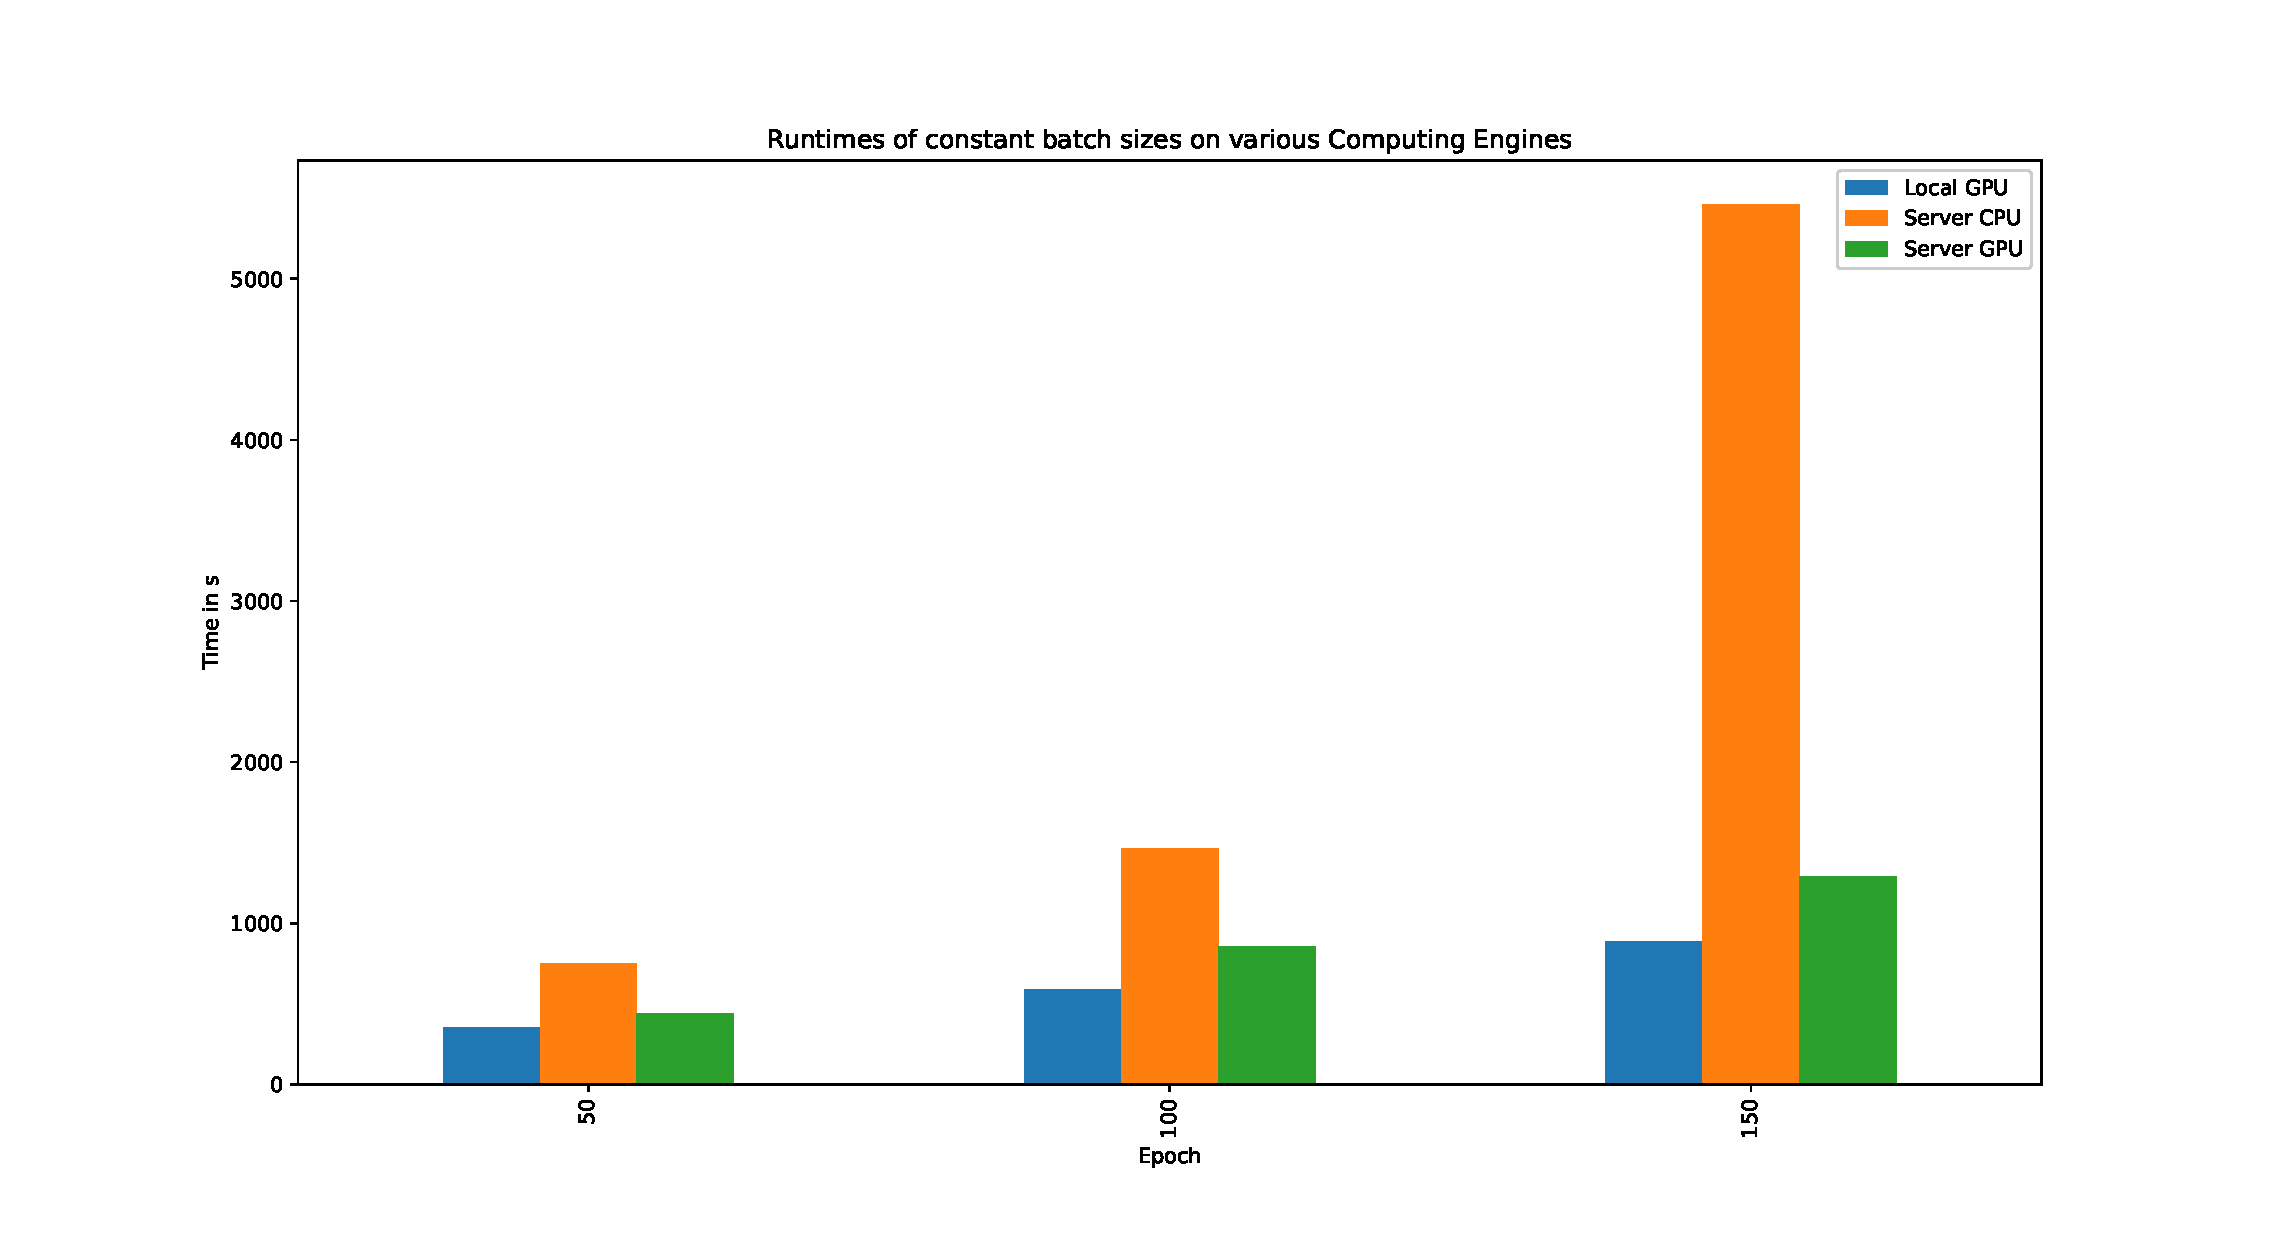
\includegraphics[width=\columnwidth]{constantbatch}
\end{centering}
\caption{Constant Batch Size (Batch Size=50)}
\end{figure}
\begin{figure}[!ht]
\begin{centering}
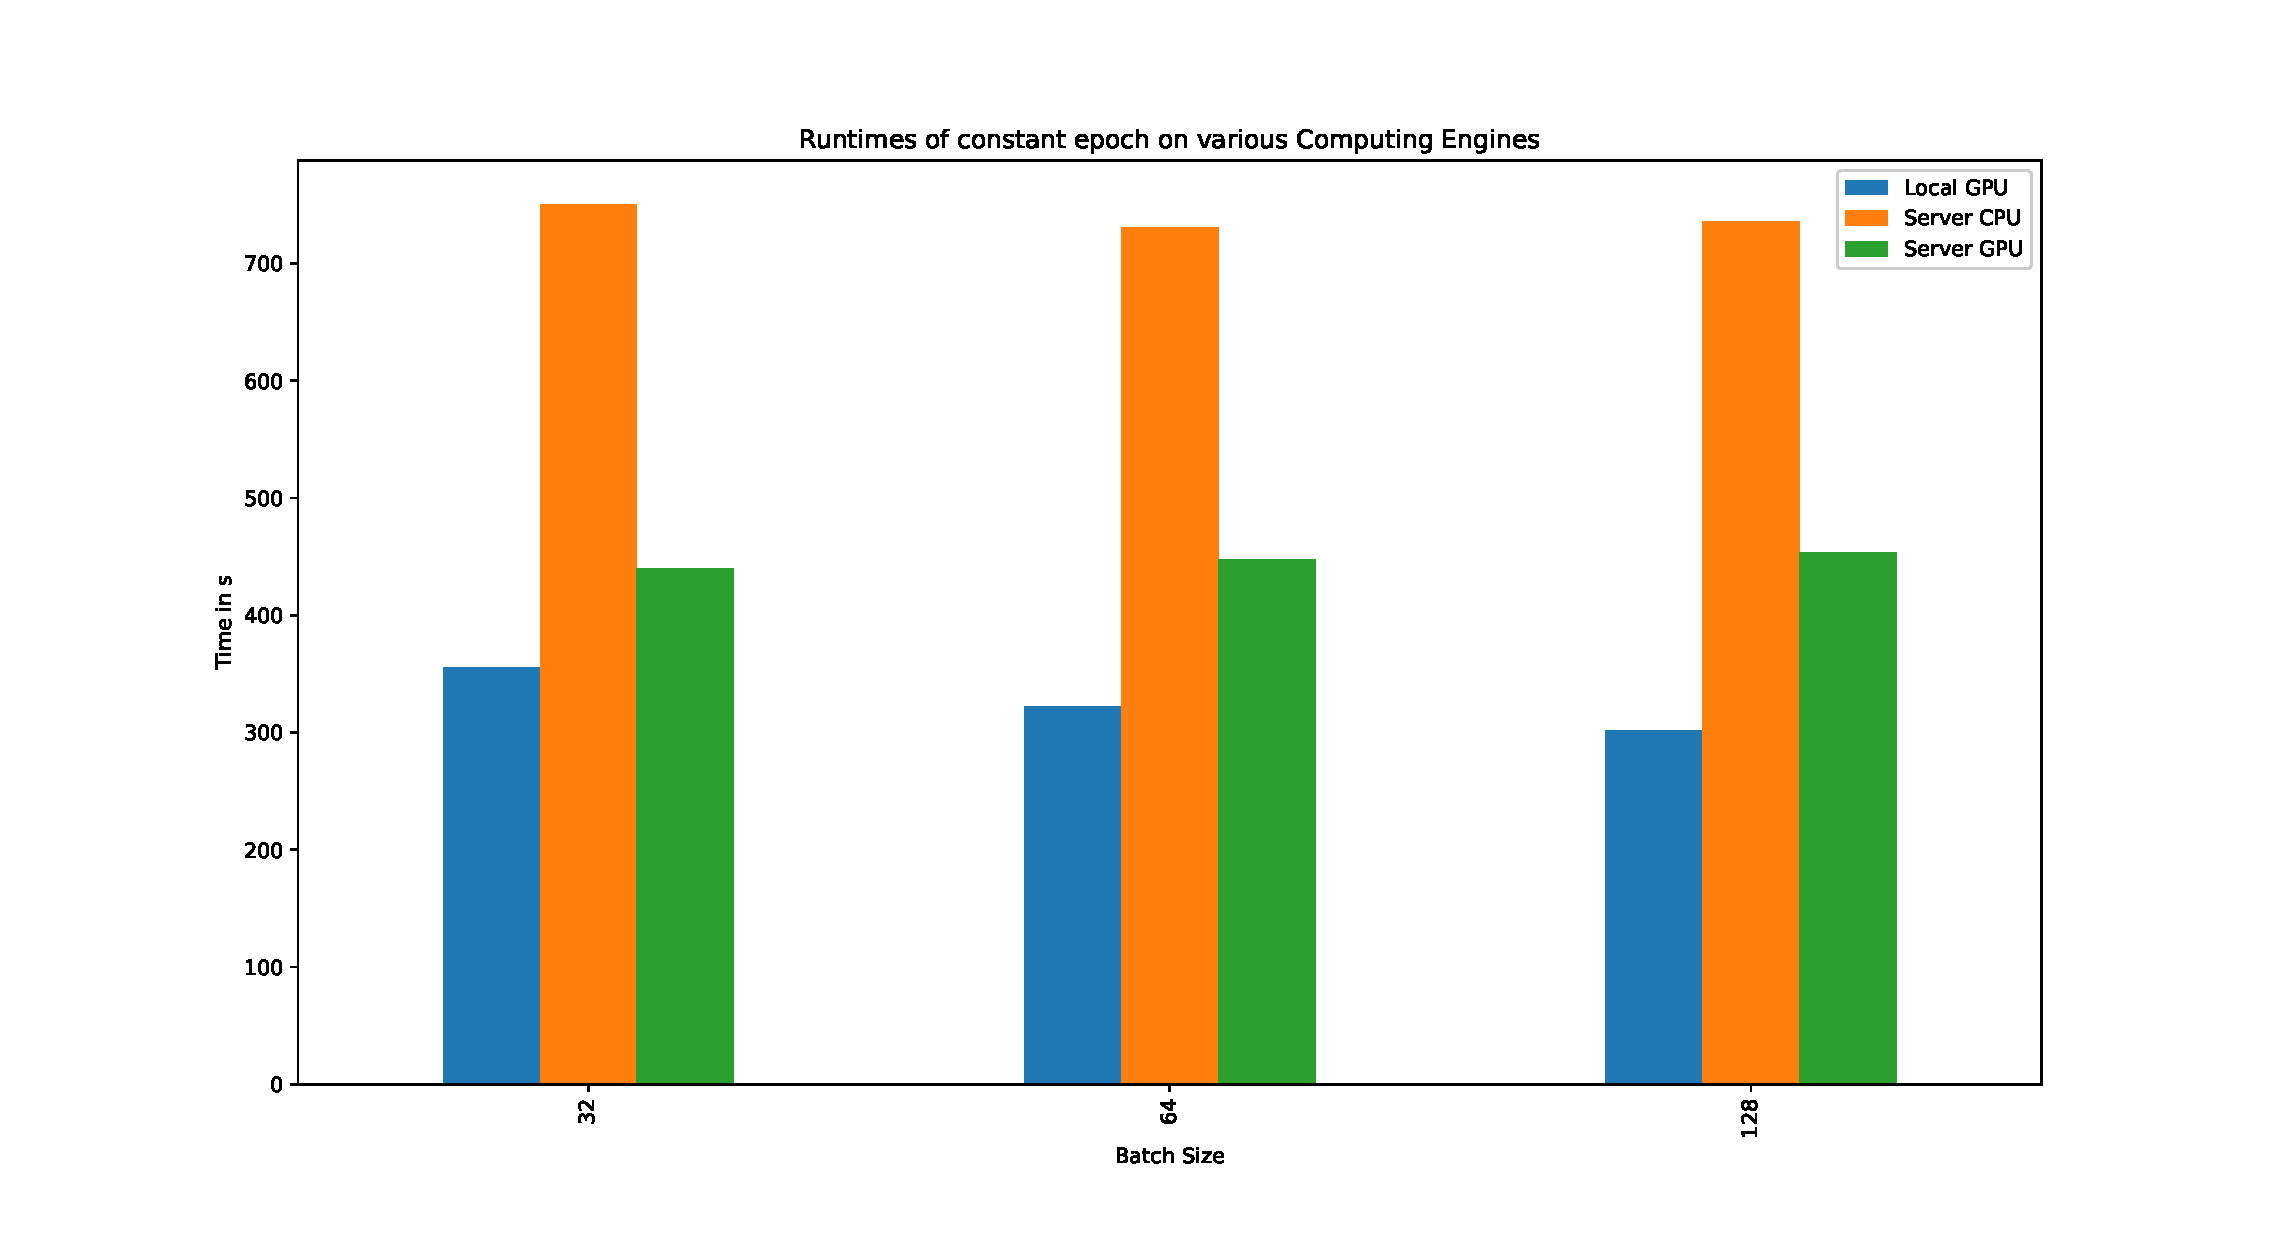
\includegraphics[width=\columnwidth]{constantepoch}
\end{centering}
\caption{Constant Epoch (Epochs=128)}
\end{figure}
\end{enumerate}
\section{Optional}
\begin{enumerate}[label=\thesection.\arabic*.,ref=\thesection.\theenumi]
\item Run runMain.py for visualizing the calculation of steering values.
\end{enumerate}
\end{document}